\sectiontitle{เฉลยและเกณฑ์ตรวจ: CPE333 Mock Midterm ชุดที่ 1}
\noindent สำหรับตรวจหลังทำข้อสอบเท่านั้น ไม่ใช่เฉลยข้อสอบจริงของรายวิชา\\คะแนนรวม 50: ปรนัย $20c/41$ เมื่อ $c$ คือจำนวนข้อถูก; เติมคำ 10; อัตนัย $8+4+8=20$\\ไม่ปัดคะแนนรายข้อ; เมื่อสรุปผลจึงปัดคะแนนรวมเป็นทศนิยมสองตำแหน่ง ไม่มีการหักคะแนนตอบผิด\par\medskip
\sectiontitle{เฉลยส่วนที่ 1: คำตอบเดียวที่ดีที่สุด}
\begin{enumerate}[leftmargin=1.4em,start=1,itemsep=0.18cm]
\item \textbf{(b)} Trap ส่งการควบคุมแบบ synchronous เข้า OS handler เช่นการร้องขอ system call ไม่ใช่ asynchronous hardware interrupt {\small [L1]}
\item \textbf{(c)} หากไม่มีการแยก privilege ผู้ใช้/process อาจเข้าถึงข้อมูลของ process อื่นหรืออุปกรณ์โดยข้ามการป้องกัน {\small [L1]}
\item \textbf{(c)} PID เป็น identifier ของ process; PCB เป็นโครงสร้างเก็บข้อมูล ไม่ใช่เลข identifier ส่วน device queue และ PFN อ้างคนละทรัพยากร {\small [L2]}
\item \textbf{(b)} Program counter ระบุตำแหน่งคำสั่งถัดไป; stack pointer ชี้ stack, page-table base ชี้ตาราง และ data register ไม่ใช่ตัวติดตามคำสั่งถัดไป {\small [L2]}
\item \textbf{(c)} Isolation แยกการเข้าถึงทรัพยากรระหว่าง applications เพื่อป้องกันการเข้าถึงที่ไม่ได้รับอนุญาต {\small [L1]}
\item \textbf{(d)} Non-preemptive/cooperative switching อาศัยงานคืน control เอง ไม่จำเป็นต้องมี timer เพื่อบังคับ preempt ตาม quantum {\small [L2]}
\item \textbf{(b)} Process descriptor/PCB เป็นข้อมูลบริหารที่ kernel เก็บรักษา ต่างจาก text/heap/stack ใน user address space {\small [L2]}
\item \textbf{(c)} ใน layout ที่เรียน heap โตขึ้นไปยัง address สูง ส่วน stack โตลงไปยัง address ต่ำ ไม่ใช่ข้อบังคับของทุก architecture {\small [L2]}
\item \textbf{(d)} Ready ไม่ได้กำลังรันเพื่อร้องขอ I/O จึงไม่มี transition ready ไป blocked โดยตรงในโมเดลนี้ {\small [L2]}
\item \textbf{(d)} Process state บอกกิจกรรม/สถานะปัจจุบัน เช่น ready/running/blocked ไม่ใช่กิจกรรมที่ผ่านมา จะทำในอนาคต หรือกิจกรรมสุดท้าย {\small [L2]}
\item \textbf{(a)} Blocked on disk read รอ event คือ I/O completion ไม่ใช่รอ timer หรือเลือก CPU {\small [L2]}
\end{enumerate}
\newpage\sectiontitle{เฉลยส่วนที่ 1 (ต่อ)}
\begin{enumerate}[leftmargin=1.4em,start=12,itemsep=0.18cm]
\item \textbf{(b)} Zombie คือจบการทำงานแล้ว แต่ parent ยังไม่เก็บ exit status ด้วย wait/waitpid {\small [L2]}
\item \textbf{(c)} PCB/process descriptor เก็บข้อมูลบริหาร process เช่น state, saved context และ scheduling information; TLB เก็บ translation, stack ใช้ call/local state และ frame เป็นพื้นที่ physical memory {\small [L2]}
\item \textbf{(d)} Parent wait สำเร็จหลัง child จบ ดังนั้นในเงื่อนไขนี้ child พิมพ์ก่อน parent โดยสมมติ output สำเร็จและไม่พิจารณา buffering ที่เปลี่ยนลำดับการแสดง {\small [L2]}
\item \textbf{(a)} FIFO/FCFS ใช้ลำดับการมาถึง ไม่ได้เรียงตามความยาวหรือ priority; แก้ stem เดิมให้ไม่กำกวมกับ RR first dispatch {\small [L3]}
\item \textbf{(d)} หลัง fork แรกมี 2 processes และทุกตัว fork อีกครั้งเป็น 4 processes จึงพิมพ์สี่ครั้ง ไม่ใช่บวกทีละหนึ่ง {\small [L2]}
\item \textbf{(a)} MLFQ ให้งานใหม่เริ่มที่ priority สูงสุด ไม่ใช่ต่ำสุด {\small [L3]}
\item \textbf{(c)} Virtual memory อนุญาตให้ address spaces ที่ใช้มีขนาดรวมเกิน RAM โดยเก็บบางส่วนใน backing storage ได้ {\small [L6]}
\item \textbf{(a)} OS สลับการใช้ CPU ให้แต่ละ process เห็นเสมือนมี CPU ของตนเอง ไม่ใช่ว่า single core รันทุก process พร้อมกันจริงหรือ fetch คำสั่งจาก disk โดยตรง {\small [L1]}
\item \textbf{(b)} Fixed partitions อาจเหลือพื้นที่ภายในหน่วยที่จัดสรร ส่วน variable partitions อาจมี external fragmentation และ compaction ไม่แก้ internal waste {\small [L4]}
\item \textbf{(c)} CPU scheduler เลือก ready process ให้ใช้ CPU ไม่ใช่เลือก victim page หรือจัดสรร frame {\small [L3]}
\item \textbf{(a)} Page replacement เลือก resident victim page เพื่อคืน frame เมื่อจำเป็นต้องแทนที่ {\small [L6]}
\end{enumerate}
\newpage\sectiontitle{เฉลยส่วนที่ 1 (ต่อ)}
\begin{enumerate}[leftmargin=1.4em,start=23,itemsep=0.18cm]
\item \textbf{(b)} exec สำเร็จแทนที่ process image จึงไม่กลับจุดเรียกเดิม ส่วน fork และ wait มี return path ตามปกติ; เติม when it succeeds เพื่อแยกกรณี exec ล้มเหลว {\small [L2]}
\item \textbf{(b)} Segments มีขนาดต่างกันและแต่ละ segment ต้องต่อเนื่อง จึงเกิด holes/external fragmentation ได้ {\small [L5]}
\item \textbf{(c)} Demand paging โหลด page เมื่อ reference แล้วพบว่ายังไม่ resident ไม่ต้องโหลดทั้ง process ก่อน {\small [L6]}
\item \textbf{(d)} Legal not-present fault โดยปกติแก้ด้วย page-in และ restart; ไม่ควร terminate ทุกกรณี ต่างจาก invalid/protection access {\small [L6]}
\item \textbf{(d)} Segment ใช้ base แปลตำแหน่งและ limit ตรวจ offset; ตัวเลือกอื่นปน paging, scheduling หรือข้อมูลที่ไม่ใช่คู่ base/bounds ของ segment {\small [L5]}
\item \textbf{(a)} Page ใหญ่ขึ้นทำให้จำนวน pages ลดลง จึงมี PTE entries น้อยลงเมื่อ address-space size และ PTE size คงที่ {\small [L5]}
\item \textbf{(d)} Non-preemptive FIFO อาศัย process จบ/block/yield ไม่ต้องใช้ timer ตัด CPU ตาม quantum {\small [L3]}
\item \textbf{(b)} Backing storage เช่น disk/swap ใช้เก็บ pages ที่ไม่ได้อยู่ใน RAM; TLB เก็บ translations ไม่ใช่เนื้อหา page {\small [L6]}
\item \textbf{(c)} Response วัดจาก arrival ถึงการเริ่มได้รับ CPU ครั้งแรก ต่างจาก turnaround และ total waiting {\small [L3]}
\item \textbf{(a)} Turnaround คือเวลาตั้งแต่ส่ง/เข้าระบบจนเสร็จสมบูรณ์ {\small [L3]}
\end{enumerate}
\newpage\sectiontitle{เฉลยส่วนที่ 1 (ต่อ)}
\begin{enumerate}[leftmargin=1.4em,start=33,itemsep=0.18cm]
\item \textbf{(d)} Variable-size contiguous allocation เกิด external fragmentation; coalescing รวม holes ที่ติดกัน และ compaction ย้าย allocated blocks เพื่อรวมพื้นที่ว่าง {\small [L4]}
\item \textbf{(b)} เมื่อ pagesize/PTEsize เท่าเดิม virtual space ใหญ่ขึ้นมี virtual pages มากขึ้น จึงต้องมี entries มากขึ้น {\small [L5]}
\item \textbf{(a)} ประหยัดได้เพราะไม่ต้องจัดสรร lower-level tables ให้ virtual regions ที่ไม่ใช้ ไม่ใช่ว่าทุกตารางว่าง {\small [L5]}
\item \textbf{(c)} SJF อาจทำให้งานยาวใน ready queue รอนานไม่สิ้นสุดหากมีงานสั้นเข้ามาต่อเนื่อง; ไม่ได้ทำให้ค่าเฉลี่ยแย่สุดทุกกรณี {\small [L3]}
\item \textbf{(d)} Segmentation ใช้ส่วน logical ขนาดต่างกัน ส่วน paging ใช้ page ขนาดเท่ากัน {\small [L5]}
\item \textbf{(b)} Pages เป็นหน่วยใน virtual address space; frames เป็นหน่วยใน physical memory ที่มีขนาดเท่ากับ pages {\small [L5]}
\item \textbf{(c)} OPT ใช้ future knowledge เลือก page ที่จะไม่ถูกใช้ไปอีกนานที่สุด จึงใช้เป็น benchmark ไม่ใช่ online policy ที่รู้อนาคตจริง {\small [L6]}
\item \textbf{(a)} Not-present legal page ทำให้ fault เพื่อ page-in; TLB hit ไม่ใช่ fault และ TLB miss ก็ไม่ได้หมายความว่า fault เสมอ {\small [L6]}
\item \textbf{(c)} RR หมุนงานตาม quantum; FIFO/SJF แบบ non-preemptive ไม่ตัดตาม slice และ OPT เป็น page replacement ไม่ใช่ CPU scheduling {\small [L3]}
\end{enumerate}
\newpage\sectiontitle{เฉลยส่วนที่ 2: เติมคำ / ตอบสั้น}
\noindent ข้อละ 1 คะแนน ให้ partial credit ตามองค์ประกอบในแต่ละข้อ; รับถ้อยคำอื่นที่มีความหมายถูกต้อง ไม่บังคับจำประโยคเฉลย\par\smallskip
\begin{enumerate}[leftmargin=1.4em,itemsep=.25cm]
\item \textbf{MLFQ: Multilevel Feedback Queue. STCF: Shortest Time-to-Completion First.}\\0.5 for each correct full name. Accept Multi-level and equivalent hyphenation.; สองคำย่อที่ใช้จริงใน Lecture 3 และโจทย์ scheduling ไม่ใช่คำย่ออุปกรณ์พื้นฐานเรียงหลายข้อ
\item \textbf{A program is passive code; a process is a program in execution.}\\0.5 for passive code; 0.5 for a program in execution. No resource list or additional explanation required.; Process ไม่ใช่แค่ไฟล์ program ใน disk; program เดียวมีหลาย process ได้
\item \textbf{Memory Management Unit; translates virtual addresses to physical addresses.}\\0.5 for the full name; 0.5 for virtual-to-physical translation. No protection details required.; แทนข้อ cooperative ที่ซ้ำปรนัย เพื่อเพิ่มคำย่อและความเข้าใจกลไกหน่วยความจำ
\item \textbf{Program counter (PC) and stack pointer (SP).}\\0.5 each for two distinct valid items, such as PC, SP, a general-purpose register, or the processor status register. No switching steps required.; ปรับจากแนว context switch ให้ถามเพียงตัวอย่าง 2 อย่าง ไม่บังคับอธิบายขั้นตอนเพิ่ม
\item \textbf{Process ID (PID) and process state.}\\0.5 each for two distinct non-register information types, such as PID, state, scheduling information, or memory-management information. No PCB expansion required.; ถามข้อมูล 2 ประเภท ไม่ถามชื่อเต็มพ่วงอีกส่วน และแยกจากตัวอย่าง register ในข้อก่อนหน้า
\end{enumerate}\newpage\sectiontitle{เฉลยส่วนที่ 2: Short Answer (ต่อ)}\begin{enumerate}[leftmargin=1.4em,start=6,itemsep=.25cm]
\item \textbf{Zombie process.}\\1 point for zombie or zombie process. No reason required; do not substitute orphan.; ข้อนี้ถาม keyword เท่านั้น ไม่หักคะแนนเพราะไม่ได้อธิบายเหตุผลที่โจทย์ไม่ได้ถาม
\item \textbf{I/O-bound: copying a large file; CPU-bound: matrix multiplication.}\\0.5 for each correctly labelled task. Accept equivalent examples under ordinary workload assumptions; no definitions or burst analysis required.; ปรับจากคำถามนิยามเป็นตัวอย่างงาน 2 ประเภท ไม่ใช้ชื่ออุปกรณ์ลอย ๆ และไม่อ้างว่าคัดถ้อยคำเดิม
\item \textbf{Long jobs delay shorter jobs, increasing average turnaround time.}\\1 point for the delay imposed on shorter jobs and its effect on the average; no claim that LJF is impossible.; LJF มีได้ แต่ไม่เหมาะกับเป้าหมาย average turnaround ของงาน batch ตามเงื่อนไขที่เรียน
\item \textbf{No; 4200 exceeds the 4096-byte bound.}\\0.5 for No; 0.5 for the correct bounds comparison. No physical-address calculation or fault-handling steps required.; ต้องตรวจ bounds ก่อนบวก base; คำตอบ 20584 เป็นการคำนวณโดยข้าม protection check
\item \textbf{Translation Lookaside Buffer; the translation may be uncached while the page is still in RAM.}\\0.5 for the full name; 0.5 for cached-translation miss versus nonresident-page distinction.; TLB เป็น cache ของ translations ไม่ใช่ page contents จึง miss ได้ทั้งที่ page ยังอยู่ RAM
\end{enumerate}\newpage\sectiontitle{เฉลยอัตนัยข้อ 1: CPU Scheduling (8 คะแนน)}
\noindent Burst = (10,1,2,1,5) ms; arrival = 0 ทุกงาน; quantum = 1 ms; เฉลยใช้ overhead 0 และให้ SJF ตัดสินงานยาวเท่ากันตามลำดับมาถึง เป็นข้อตกลงในการทำเฉลย ไม่ใช่ข้อความที่เพิ่มในโจทย์ รับลำดับ tie อื่นที่สอดคล้องกับ SJF และคำนวณถูกต้อง\par
\noindent\textbf{FIFO}
\begin{center}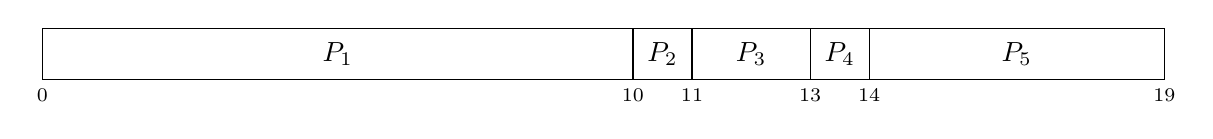
\begin{tikzpicture}[x=0.75cm,y=0.65cm]
\draw (0,0) rectangle (10,1);\node at (5.0,.5) {$P_1$};
\draw (10,0) rectangle (11,1);\node at (10.5,.5) {$P_2$};
\draw (11,0) rectangle (13,1);\node at (12.0,.5) {$P_3$};
\draw (13,0) rectangle (14,1);\node at (13.5,.5) {$P_4$};
\draw (14,0) rectangle (19,1);\node at (16.5,.5) {$P_5$};
\node[below,font=\scriptsize] at (0,0) {0};
\node[below,font=\scriptsize] at (10,0) {10};
\node[below,font=\scriptsize] at (11,0) {11};
\node[below,font=\scriptsize] at (13,0) {13};
\node[below,font=\scriptsize] at (14,0) {14};
\node[below,font=\scriptsize] at (19,0) {19};
\end{tikzpicture}\end{center}
\noindent\textbf{SJF}
\begin{center}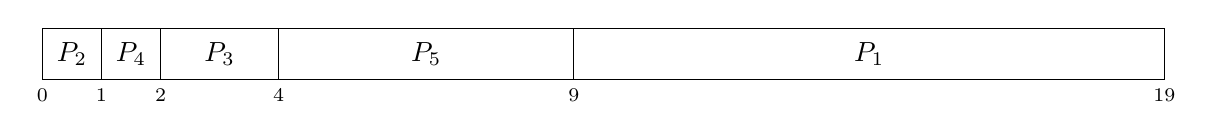
\begin{tikzpicture}[x=0.75cm,y=0.65cm]
\draw (0,0) rectangle (1,1);\node at (0.5,.5) {$P_2$};
\draw (1,0) rectangle (2,1);\node at (1.5,.5) {$P_4$};
\draw (2,0) rectangle (4,1);\node at (3.0,.5) {$P_3$};
\draw (4,0) rectangle (9,1);\node at (6.5,.5) {$P_5$};
\draw (9,0) rectangle (19,1);\node at (14.0,.5) {$P_1$};
\node[below,font=\scriptsize] at (0,0) {0};
\node[below,font=\scriptsize] at (1,0) {1};
\node[below,font=\scriptsize] at (2,0) {2};
\node[below,font=\scriptsize] at (4,0) {4};
\node[below,font=\scriptsize] at (9,0) {9};
\node[below,font=\scriptsize] at (19,0) {19};
\end{tikzpicture}\end{center}
\noindent\textbf{RR}
\begin{center}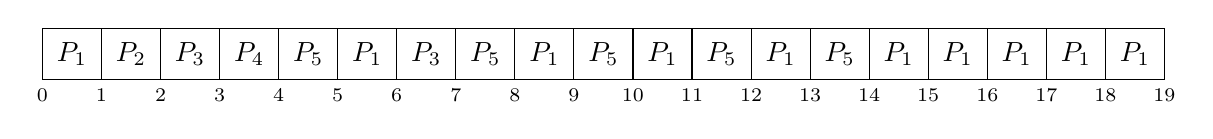
\begin{tikzpicture}[x=0.75cm,y=0.65cm]
\draw (0,0) rectangle (1,1);\node at (0.5,.5) {$P_1$};
\draw (1,0) rectangle (2,1);\node at (1.5,.5) {$P_2$};
\draw (2,0) rectangle (3,1);\node at (2.5,.5) {$P_3$};
\draw (3,0) rectangle (4,1);\node at (3.5,.5) {$P_4$};
\draw (4,0) rectangle (5,1);\node at (4.5,.5) {$P_5$};
\draw (5,0) rectangle (6,1);\node at (5.5,.5) {$P_1$};
\draw (6,0) rectangle (7,1);\node at (6.5,.5) {$P_3$};
\draw (7,0) rectangle (8,1);\node at (7.5,.5) {$P_5$};
\draw (8,0) rectangle (9,1);\node at (8.5,.5) {$P_1$};
\draw (9,0) rectangle (10,1);\node at (9.5,.5) {$P_5$};
\draw (10,0) rectangle (11,1);\node at (10.5,.5) {$P_1$};
\draw (11,0) rectangle (12,1);\node at (11.5,.5) {$P_5$};
\draw (12,0) rectangle (13,1);\node at (12.5,.5) {$P_1$};
\draw (13,0) rectangle (14,1);\node at (13.5,.5) {$P_5$};
\draw (14,0) rectangle (15,1);\node at (14.5,.5) {$P_1$};
\draw (15,0) rectangle (16,1);\node at (15.5,.5) {$P_1$};
\draw (16,0) rectangle (17,1);\node at (16.5,.5) {$P_1$};
\draw (17,0) rectangle (18,1);\node at (17.5,.5) {$P_1$};
\draw (18,0) rectangle (19,1);\node at (18.5,.5) {$P_1$};
\node[below,font=\scriptsize] at (0,0) {0};
\node[below,font=\scriptsize] at (1,0) {1};
\node[below,font=\scriptsize] at (2,0) {2};
\node[below,font=\scriptsize] at (3,0) {3};
\node[below,font=\scriptsize] at (4,0) {4};
\node[below,font=\scriptsize] at (5,0) {5};
\node[below,font=\scriptsize] at (6,0) {6};
\node[below,font=\scriptsize] at (7,0) {7};
\node[below,font=\scriptsize] at (8,0) {8};
\node[below,font=\scriptsize] at (9,0) {9};
\node[below,font=\scriptsize] at (10,0) {10};
\node[below,font=\scriptsize] at (11,0) {11};
\node[below,font=\scriptsize] at (12,0) {12};
\node[below,font=\scriptsize] at (13,0) {13};
\node[below,font=\scriptsize] at (14,0) {14};
\node[below,font=\scriptsize] at (15,0) {15};
\node[below,font=\scriptsize] at (16,0) {16};
\node[below,font=\scriptsize] at (17,0) {17};
\node[below,font=\scriptsize] at (18,0) {18};
\node[below,font=\scriptsize] at (19,0) {19};
\end{tikzpicture}\end{center}
\noindent RR ยังคงมีจุดแบ่ง quantum แม้เหลือเพียง $P_1$; จะรวมช่วงติดกันของ $P_1$ ตอนท้ายก็ได้ถ้าระบุ quantum ถูกต้อง\par\medskip
\noindent\textbf{นิยามที่ใช้}\\$T_i=C_i-A_i$; $R_i=S_i-A_i$; $W_i=T_i-B_i$ (กรณีมี CPU burst เดียว ไม่มี I/O)\\$C$: completion, $A$: arrival, $S$: first start, $B$: CPU burst\\Response time ไม่ใช่ total waiting time โดยเฉพาะเมื่อใช้ RR\par
\newpage\sectiontitle{เฉลยอัตนัยข้อ 1 (ต่อ): ตารางและเกณฑ์ตรวจ}
\noindent\textbf{Turnaround time (ms)}
\begin{center}\renewcommand{\arraystretch}{1.15}\begin{tabular}{lrrrrr}
Policy & $P_1$ & $P_2$ & $P_3$ & $P_4$ & $P_5$\\\hline
FIFO & 10 & 11 & 13 & 14 & 19\\
SJF & 19 & 1 & 4 & 2 & 9\\
RR & 19 & 2 & 7 & 4 & 14\\
\end{tabular}\end{center}
\noindent\textbf{Response time (ms)}
\begin{center}\renewcommand{\arraystretch}{1.15}\begin{tabular}{lrrrrr}
Policy & $P_1$ & $P_2$ & $P_3$ & $P_4$ & $P_5$\\\hline
FIFO & 0 & 10 & 11 & 13 & 14\\
SJF & 9 & 0 & 2 & 1 & 4\\
RR & 0 & 1 & 2 & 3 & 4\\
\end{tabular}\end{center}
\noindent\textbf{Waiting time (ms) - เพิ่มเพื่อเทียบ ไม่ได้ถามให้คำนวณ}
\begin{center}\renewcommand{\arraystretch}{1.15}\begin{tabular}{lrrrrr}
Policy & $P_1$ & $P_2$ & $P_3$ & $P_4$ & $P_5$\\\hline
FIFO & 0 & 10 & 11 & 13 & 14\\
SJF & 9 & 0 & 2 & 1 & 4\\
RR & 9 & 1 & 5 & 3 & 9\\
\end{tabular}\end{center}
\begin{center}\renewcommand{\arraystretch}{1.15}\begin{tabular}{lrr}
Policy & Average turnaround & Average response\\\hline
FIFO & 13.4 ms & 9.6 ms\\
SJF & 7.0 ms & 3.2 ms\\
RR & 9.2 ms & 2.0 ms\\
\end{tabular}\end{center}
\noindent\textbf{สรุป:} SJF ให้ average turnaround ต่ำสุด 7.0 ms; RR ให้ average response ต่ำสุด 2.0 ms สำหรับ workload นี้เท่านั้น\par\medskip
\noindent\textbf{Rubric รวม 8 คะแนน}
\begin{itemize}[leftmargin=1.4em,itemsep=.12cm]
\item (a) 3 คะแนน: FIFO, SJF, RR อย่างละ 1; แต่ละอันให้ .5 สำหรับลำดับและ .5 สำหรับขอบเวลาถูกต้อง
\item (b) 2 คะแนน: ตาราง turnaround 15 ค่า ค่าละ $2/15$ คะแนน
\item (c) 2 คะแนน: ตาราง response 15 ค่า ค่าละ $2/15$ คะแนน
\item (d) 1 คะแนน: เลือก SJF สำหรับ minimum average Turnaround .5 และ RR สำหรับ minimum average Response .5; ตารางค่าเฉลี่ยทั้ง 6 ค่าแสดงไว้สำหรับตรวจทบทวน ไม่บังคับรายงานทุกค่าที่โจทย์ไม่ได้ถาม
\end{itemize}
\noindent หากผิดจาก arithmetic ครั้งเดียวแต่ขั้นถัดไปใช้วิธีถูก ให้ follow-through credit โดยไม่หักซ้ำ; ไม่ให้ครบในส่วนที่ใช้นิยาม response ผิดเป็น waiting
\newpage\sectiontitle{เฉลยอัตนัยข้อ 2: MLFQ กับธนาคาร (4 คะแนน)}
\noindent\textbf{เกณฑ์ตรวจภาพรวม: กฎ MLFQ และการเทียบกับธนาคาร (2 คะแนน; ข้อละ .4)}
\begin{enumerate}[leftmargin=1.4em,itemsep=.18cm]
\item Priority สูงกว่าจะได้บริการก่อน: เลือกคิวระดับสูงสุดที่มีลูกค้าพร้อมทำรายการ
\item Priority เท่ากันใช้ RR: ให้บริการเป็นช่วงแล้วหมุนเวียนเมื่อถึงจุดพักที่ปลอดภัย หากยังทำไม่เสร็จ
\item งานใหม่เริ่มที่คิวบนสุด: ลูกค้าใหม่มีโอกาสจบรายการสั้นเร็ว โดยยังไม่ต้องรู้ service time ล่วงหน้า
\item เมื่อใช้ allotment สะสมของระดับนั้นครบ ให้ลด priority หนึ่งระดับ แม้เคยพัก/yield ก่อนหมด slice; ระดับล่างสุดคงอยู่ระดับเดิม
\item ทุกช่วงเวลา $S$ ให้ boost งานที่ยังไม่เสร็จกลับคิวบนสุด ป้องกันงานยาวอดรอ และรองรับพฤติกรรมงานที่เปลี่ยนไป
\end{enumerate}
\noindent\textbf{ตัวอย่าง policy ที่ใช้งานได้ (1 คะแนน)}\\
ตัวเลขและจำนวนระดับต่อไปนี้เป็นตัวอย่าง ไม่ใช่ค่าที่โจทย์บังคับ; ให้คะแนนจากความสอดคล้องของ policy และการใช้ feedback ไม่ใช่การใช้ตัวเลขเหมือนเฉลย
\begin{itemize}[leftmargin=1.4em,itemsep=.12cm]
\item ใช้ Q0, Q1, Q2 ตามลำดับสูงไปต่ำ; slice เท่ากับ 2, 4, 8 นาที; allotment ของ Q0/Q1 เท่ากับ 2/4 นาที ส่วน Q2 หมุน RR จนจบ (.25)
\item ลูกค้าใหม่เข้า Q0, จบรายการสั้นก็ออกจากระบบ; งานที่ใช้เวลาใน Q0 สะสมครบ 2 นาทีลง Q1 และครบ 4 นาทีใน Q1 ลง Q2 (.25)
\item เมื่องาน priority สูงกว่ามาถึง ให้พักงานต่ำกว่า ณ safe stage boundary ถัดไป บันทึก progress และเวลาสะสมไว้ ไม่เริ่ม financial update ค้างครึ่งทาง (.25)
\item ตั้ง boost เช่นทุก 20 นาที และคงลำดับเข้าคิวอย่างเป็นธรรม; งาน blocked รอเอกสารไม่ควรยึด counter เมื่อกลับมาพร้อมต้องใช้กติกา boost/accounting ที่ประกาศชัด (.25)
\end{itemize}
\noindent\textbf{ข้อเสนอปรับปรุงและผลต่อ turnaround (1 คะแนน)}\\
ให้ .5 สำหรับข้อเสนอเช่นคัดกรองรายการ, จัดเตรียมเอกสารล่วงหน้า, ลด slice ในคิวสูง, เพิ่ม counter ตามกำลังคน หรือปรับ boost จากข้อมูลเวลารอจริง; อีก .5 สำหรับผลและข้อจำกัด เช่น slice สั้นเพิ่ม overhead, boost ถี่รบกวนงานสั้น, เพิ่ม counter เปลี่ยนเป็นหลาย server และมีต้นทุนเพิ่ม
\par\medskip
\noindent MLFQ ไม่ได้รับประกัน average turnaround ต่ำสุดทุก workload เพราะไม่ทราบความยาวงานล่วงหน้า และธนาคารจริงไม่สามารถ preempt ทุกจุดเหมือน CPU ได้; รับ policy อื่นที่ครบกฎและอธิบายความเป็นไปได้อย่างสอดคล้อง
\newpage\sectiontitle{เฉลยอัตนัยข้อ 3: Page Replacement (8 คะแนน)}
\noindent\textbf{ตาราง FIFO, LRU และ OPT (6 คะแนน)}\\
เฉลยเริ่มด้วย frames ว่าง แสดงสถานะหลังแต่ละ reference; F = fault, H = hit, -- = frame ว่าง เป็นสัญลักษณ์ช่วยตรวจ ไม่บังคับเพิ่มแถว H/F ในคำตอบ\par\smallskip

\noindent\textbf{FIFO: 13 faults, 7 hits}
{\setlength{\tabcolsep}{5pt}\begin{center}\renewcommand{\arraystretch}{1.15}\begin{tabular}{l|cccccccccc}
Ref. no. & 1 & 2 & 3 & 4 & 5 & 6 & 7 & 8 & 9 & 10\\\hline
Page & 7 & 0 & 1 & 3 & 0 & 3 & 2 & 4 & 2 & 7\\
Frame 1 & 7 & 7 & 7 & 3 & 3 & 3 & 3 & 3 & 3 & 7\\
Frame 2 & -- & 0 & 0 & 0 & 0 & 0 & 2 & 2 & 2 & 2\\
Frame 3 & -- & -- & 1 & 1 & 1 & 1 & 1 & 4 & 4 & 4\\
H/F & F & F & F & F & H & H & F & F & H & F\\
\end{tabular}\end{center}}
{\setlength{\tabcolsep}{5pt}\begin{center}\renewcommand{\arraystretch}{1.15}\begin{tabular}{l|cccccccccc}
Ref. no. & 11 & 12 & 13 & 14 & 15 & 16 & 17 & 18 & 19 & 20\\\hline
Page & 0 & 3 & 2 & 1 & 2 & 0 & 1 & 4 & 0 & 1\\
Frame 1 & 7 & 7 & 2 & 2 & 2 & 2 & 2 & 4 & 4 & 4\\
Frame 2 & 0 & 0 & 0 & 1 & 1 & 1 & 1 & 1 & 1 & 1\\
Frame 3 & 4 & 3 & 3 & 3 & 3 & 0 & 0 & 0 & 0 & 0\\
H/F & F & F & F & F & H & F & H & F & H & H\\
\end{tabular}\end{center}}
\noindent\textbf{LRU: 13 faults, 7 hits}
{\setlength{\tabcolsep}{5pt}\begin{center}\renewcommand{\arraystretch}{1.15}\begin{tabular}{l|cccccccccc}
Ref. no. & 1 & 2 & 3 & 4 & 5 & 6 & 7 & 8 & 9 & 10\\\hline
Page & 7 & 0 & 1 & 3 & 0 & 3 & 2 & 4 & 2 & 7\\
Frame 1 & 7 & 7 & 7 & 3 & 3 & 3 & 3 & 3 & 3 & 7\\
Frame 2 & -- & 0 & 0 & 0 & 0 & 0 & 0 & 4 & 4 & 4\\
Frame 3 & -- & -- & 1 & 1 & 1 & 1 & 2 & 2 & 2 & 2\\
H/F & F & F & F & F & H & H & F & F & H & F\\
\end{tabular}\end{center}}
{\setlength{\tabcolsep}{5pt}\begin{center}\renewcommand{\arraystretch}{1.15}\begin{tabular}{l|cccccccccc}
Ref. no. & 11 & 12 & 13 & 14 & 15 & 16 & 17 & 18 & 19 & 20\\\hline
Page & 0 & 3 & 2 & 1 & 2 & 0 & 1 & 4 & 0 & 1\\
Frame 1 & 7 & 7 & 2 & 2 & 2 & 2 & 2 & 4 & 4 & 4\\
Frame 2 & 0 & 0 & 0 & 1 & 1 & 1 & 1 & 1 & 1 & 1\\
Frame 3 & 2 & 3 & 3 & 3 & 3 & 0 & 0 & 0 & 0 & 0\\
H/F & F & F & F & F & H & F & H & F & H & H\\
\end{tabular}\end{center}}
\newpage\sectiontitle{เฉลยอัตนัยข้อ 3: ตาราง OPT (ต่อ)}
\noindent\textbf{OPT: 10 faults, 10 hits}
{\setlength{\tabcolsep}{5pt}\begin{center}\renewcommand{\arraystretch}{1.15}\begin{tabular}{l|cccccccccc}
Ref. no. & 1 & 2 & 3 & 4 & 5 & 6 & 7 & 8 & 9 & 10\\\hline
Page & 7 & 0 & 1 & 3 & 0 & 3 & 2 & 4 & 2 & 7\\
Frame 1 & 7 & 7 & 7 & 7 & 7 & 7 & 7 & 7 & 7 & 7\\
Frame 2 & -- & 0 & 0 & 0 & 0 & 0 & 0 & 4 & 4 & 4\\
Frame 3 & -- & -- & 1 & 3 & 3 & 3 & 2 & 2 & 2 & 2\\
H/F & F & F & F & F & H & H & F & F & H & H\\
\end{tabular}\end{center}}
{\setlength{\tabcolsep}{5pt}\begin{center}\renewcommand{\arraystretch}{1.15}\begin{tabular}{l|cccccccccc}
Ref. no. & 11 & 12 & 13 & 14 & 15 & 16 & 17 & 18 & 19 & 20\\\hline
Page & 0 & 3 & 2 & 1 & 2 & 0 & 1 & 4 & 0 & 1\\
Frame 1 & 0 & 0 & 0 & 0 & 0 & 0 & 0 & 0 & 0 & 0\\
Frame 2 & 4 & 3 & 3 & 1 & 1 & 1 & 1 & 1 & 1 & 1\\
Frame 3 & 2 & 2 & 2 & 2 & 2 & 2 & 2 & 4 & 4 & 4\\
H/F & F & F & H & F & H & H & H & F & H & H\\
\end{tabular}\end{center}}
\noindent ตารางตัวอย่าง OPT เลือก frame ต่ำสุดเมื่อตัดสินเสมอ; โจทย์ไม่บังคับ tie-break จึงรับ trace อื่นที่เลือกเหยื่อ optimal และได้จำนวน fault ถูกต้อง\par
\newpage\sectiontitle{เฉลยอัตนัยข้อ 3 (ต่อ): EAT และเกณฑ์ตรวจ}
\noindent\textbf{หน่วยและโมเดลต้นทุน}\\
$m=10$ ns $=0.00001$ ms; $D=10$ ms $=10{,}000{,}000$ ns\\
ใช้โมเดล Lecture 6 หน้า 29 โดยให้ $D$ แทน disk access time:
\[\mathrm{EAT}=(1-p)m+pD\]
โจทย์ต้นฉบับไม่ได้เพิ่มเงื่อนไข complete fault-path cost หรือ restarted access; สูตรนี้อิงโมเดลในสไลด์ ไม่ใช่การเติมถ้อยคำดังกล่าวลงในโจทย์

\noindent\textbf{EAT (2 คะแนน)}\\จำนวน faults, hits และ probability ด้านล่างเป็นค่าช่วยคำนวณ EAT ไม่ใช่ข้อย่อยเพิ่มในโจทย์
\begin{center}\renewcommand{\arraystretch}{1.15}\begin{tabular}{lrrrr}
Policy & Faults & Hits & p & EAT (ms)\\\hline
FIFO & 13 & 7 & 13/20 & 6.5000035\\
LRU & 13 & 7 & 13/20 & 6.5000035\\
OPT & 10 & 10 & 10/20 & 5.0000050\\
\end{tabular}\end{center}
\[\mathrm{EAT}_{FIFO}=\mathrm{EAT}_{LRU}=\frac7{20}(10)+\frac{13}{20}(10{,}000{,}000)=6{,}500{,}003.5\ \mathrm{ns}\]
\[\mathrm{EAT}_{OPT}=\frac{10}{20}(10)+\frac{10}{20}(10{,}000{,}000)=5{,}000{,}005\ \mathrm{ns}\]
\noindent ดังนั้น OPT ต่ำสุด; FIFO กับ LRU เท่ากันสำหรับ string นี้ ไม่ได้หมายความว่าจะเท่ากันสำหรับ string อื่น\\รับคำตอบประมาณ 6.5 ms และ 5.0 ms เมื่อมีสูตรและหน่วยถูกต้อง; อย่าใช้ $10^{-3}$ วินาทีแทน 10 ms ซึ่งจริง ๆ เท่ากับ $10^{-2}$ วินาที
\par\medskip
\noindent\textbf{Rubric รวม 8 คะแนน}
\begin{itemize}[leftmargin=1.4em,itemsep=.18cm]
\item ตาราง frames รวม 6 คะแนน: แต่ละ policy 2 คะแนน ให้ตาม frame contents 20 คอลัมน์ คอลัมน์ละ .1; ไม่หักเพราะไม่มีแถว hit/fault หรือการรายงาน counts แยกต่างหาก
\item EAT รวม 2 คะแนน: สูตร .5; แปลงหน่วย .5; EAT แต่ละ policy ค่าละ $1/3$ ไม่บังคับเขียนข้อสรุปเพิ่มเติมที่โจทย์ไม่ได้ถาม
\end{itemize}
\noindent ให้ follow-through credit สำหรับ EAT ที่ใช้จำนวน fault จากตารางของผู้สอบอย่างถูกวิธี แม้ตารางก่อนหน้าผิด โดยหักข้อผิดเดิมในตาราง/จำนวน faults; ต้องไม่ให้คะแนนเต็มหากแทนค่าคนละหน่วยในสมการเดียวกัน
\newpage\sectiontitle{แผนผังเนื้อหาและแหล่งอ้างอิงสำหรับตรวจทบทวน}
\noindent\textbf{ความครอบคลุมของปรนัย}

\begin{center}\renewcommand{\arraystretch}{1.15}\begin{tabular}{lcl}
Lecture & จำนวนปรนัย & หัวข้อ\\\hline
1 & 4 & Privilege, trap, isolation\\
2 & 13 & Process, state, context switch, wait\\
3 & 8 & FIFO/SJF/STCF/RR, MLFQ, metrics\\
4 & 2 & Fixed/variable partitions, fragmentation\\
5 & 7 & Segmentation, paging, address translation\\
6 & 7 & Virtual memory, demand paging, replacement\\
\end{tabular}\end{center}
\noindent\textbf{แหล่งเนื้อหา (path เทียบกับ root ของ repository)}
\begin{itemize}[leftmargin=1.4em,itemsep=.18cm]
\item lectures/CPE333\_OS\_Midterm\_StudyNotes.pdf และ Lecture1--Lecture6: ใช้กำหนดขอบเขต ไม่รวม threads/locks/deadlock ที่อยู่นอกชุด Lecture 1--6
\item ปรนัย 5 ข้ออิงปี 2561 (E03) และ 36 ข้ออิงปี 2022 (E05) มีเลขข้อ/หน้าต้นทางใน SOURCE\_MAP.md และ question-bank.json; E09 เป็นชุดเนื้อหาซ้ำสำหรับเทียบตัวเลือก ไม่ใช้ annotation เป็นเฉลย
\item quiz-and-exam/midterm/Backroom.pdf และข้อสอบปี 2558/2561: เทียบหัวข้อและแนวคำถาม ไม่คัดลอกหน้าที่มีคำตอบเขียนกำกับ
\item quiz-and-exam/midterm/ยำรวมมิตรข้อเขียน.pdf หน้า 4--6 และ 10: Scheduling, bank analogy และ MLFQ rules; ตัวเลข burst ใช้ 10,1,2,1,5 รวม 19 ms ตามโจทย์ชุดนี้ ไม่ใช่ Quiz อีกชุดที่ $P_4=2$
\item E05: OS-Midterm-2022 ไฟล์ชื่อยาว หน้า 2 ใช้ reference string 20 ตัว, 3 frames, 10 ns/10 ms; หน้า 3--6 เป็นภาพปรนัยถึงข้อ 51 ส่วนหน้าสรุป 7--9 มีถึงข้อ 40 เท่านั้น
\item quiz-and-exam/midterm/Quiz\_BeforeMidterm.pdf: เทียบรูปแบบโจทย์ Scheduling และ fit policy
\end{itemize}
\noindent\textbf{แม่แบบการพิมพ์}\\
Palapluem/cpe222-past-exam-main, commit e87b379d09fdeb54f964d968c9599efdea68ba5d; main wrapper, cover และ chapter templates\\
คงการประกอบ PDF, ฟอนต์ THSarabunNew, margin, student header และกล่องหน้าปก; บรรทัดดอกจันบนปกใช้ข้อความตามแม่แบบที่ผู้ใช้ขอ ไม่ใช่การตรวจยืนยันการรับรองจริง
\par\medskip
\noindent วันและเวลาตามข้อมูลที่ผู้ใช้ให้: 26 ตุลาคม 2569, 09.00--12.00 น. รายละเอียดคะแนนย่อยและเฉลยเป็นเกณฑ์ฝึกซ้อมแยกเล่ม ดู README.md และ question-bank.json สำหรับ provenance
